\documentclass[twoside]{book}

% Packages required by doxygen
\usepackage{fixltx2e}
\usepackage{calc}
\usepackage{doxygen}
\usepackage[export]{adjustbox} % also loads graphicx
\usepackage{graphicx}
\usepackage[utf8]{inputenc}
\usepackage{makeidx}
\usepackage{multicol}
\usepackage{multirow}
\PassOptionsToPackage{warn}{textcomp}
\usepackage{textcomp}
\usepackage[nointegrals]{wasysym}
\usepackage[table]{xcolor}

% Font selection
\usepackage[T1]{fontenc}
\usepackage[scaled=.90]{helvet}
\usepackage{courier}
\usepackage{amssymb}
\usepackage{sectsty}
\renewcommand{\familydefault}{\sfdefault}
\allsectionsfont{%
  \fontseries{bc}\selectfont%
  \color{darkgray}%
}
\renewcommand{\DoxyLabelFont}{%
  \fontseries{bc}\selectfont%
  \color{darkgray}%
}
\newcommand{\+}{\discretionary{\mbox{\scriptsize$\hookleftarrow$}}{}{}}

% Page & text layout
\usepackage{geometry}
\geometry{%
  a4paper,%
  top=2.5cm,%
  bottom=2.5cm,%
  left=2.5cm,%
  right=2.5cm%
}
\tolerance=750
\hfuzz=15pt
\hbadness=750
\setlength{\emergencystretch}{15pt}
\setlength{\parindent}{0cm}
\setlength{\parskip}{3ex plus 2ex minus 2ex}
\makeatletter
\renewcommand{\paragraph}{%
  \@startsection{paragraph}{4}{0ex}{-1.0ex}{1.0ex}{%
    \normalfont\normalsize\bfseries\SS@parafont%
  }%
}
\renewcommand{\subparagraph}{%
  \@startsection{subparagraph}{5}{0ex}{-1.0ex}{1.0ex}{%
    \normalfont\normalsize\bfseries\SS@subparafont%
  }%
}
\makeatother

% Headers & footers
\usepackage{fancyhdr}
\pagestyle{fancyplain}
\fancyhead[LE]{\fancyplain{}{\bfseries\thepage}}
\fancyhead[CE]{\fancyplain{}{}}
\fancyhead[RE]{\fancyplain{}{\bfseries\leftmark}}
\fancyhead[LO]{\fancyplain{}{\bfseries\rightmark}}
\fancyhead[CO]{\fancyplain{}{}}
\fancyhead[RO]{\fancyplain{}{\bfseries\thepage}}
\fancyfoot[LE]{\fancyplain{}{}}
\fancyfoot[CE]{\fancyplain{}{}}
\fancyfoot[RE]{\fancyplain{}{\bfseries\scriptsize Generated by Doxygen }}
\fancyfoot[LO]{\fancyplain{}{\bfseries\scriptsize Generated by Doxygen }}
\fancyfoot[CO]{\fancyplain{}{}}
\fancyfoot[RO]{\fancyplain{}{}}
\renewcommand{\footrulewidth}{0.4pt}
\renewcommand{\chaptermark}[1]{%
  \markboth{#1}{}%
}
\renewcommand{\sectionmark}[1]{%
  \markright{\thesection\ #1}%
}

% Indices & bibliography
\usepackage{natbib}
\usepackage[titles]{tocloft}
\setcounter{tocdepth}{3}
\setcounter{secnumdepth}{5}
\makeindex

% Hyperlinks (required, but should be loaded last)
\usepackage{ifpdf}
\ifpdf
  \usepackage[pdftex,pagebackref=true]{hyperref}
\else
  \usepackage[ps2pdf,pagebackref=true]{hyperref}
\fi
\hypersetup{%
  colorlinks=true,%
  linkcolor=blue,%
  citecolor=blue,%
  unicode%
}

% Custom commands
\newcommand{\clearemptydoublepage}{%
  \newpage{\pagestyle{empty}\cleardoublepage}%
}

\usepackage{caption}
\captionsetup{labelsep=space,justification=centering,font={bf},singlelinecheck=off,skip=4pt,position=top}

%===== C O N T E N T S =====

\begin{document}

% Titlepage & ToC
\hypersetup{pageanchor=false,
             bookmarksnumbered=true,
             pdfencoding=unicode
            }
\pagenumbering{alph}
\begin{titlepage}
\vspace*{7cm}
\begin{center}%
{\Large 04-\/doxygen }\\
\vspace*{1cm}
{\large Generated by Doxygen 1.8.13}\\
\end{center}
\end{titlepage}
\clearemptydoublepage
\pagenumbering{roman}
\tableofcontents
\clearemptydoublepage
\pagenumbering{arabic}
\hypersetup{pageanchor=true}

%--- Begin generated contents ---
\chapter{Hierarchical Index}
\section{Class Hierarchy}
This inheritance list is sorted roughly, but not completely, alphabetically\+:\begin{DoxyCompactList}
\item \contentsline{section}{bayan\+:\+:hash\+:\+:hash}{\pageref{classbayan_1_1hash_1_1hash}}{}
\begin{DoxyCompactList}
\item \contentsline{section}{bayan\+:\+:hash\+:\+:md5}{\pageref{classbayan_1_1hash_1_1md5}}{}
\end{DoxyCompactList}
\item \contentsline{section}{bayan\+:\+:options}{\pageref{structbayan_1_1options}}{}
\end{DoxyCompactList}

\chapter{Class Index}
\section{Class List}
Here are the classes, structs, unions and interfaces with brief descriptions\+:\begin{DoxyCompactList}
\item\contentsline{section}{\hyperlink{classedu__allocator}{edu\+\_\+allocator$<$ T, batch\+\_\+count $>$} }{\pageref{classedu__allocator}}{}
\item\contentsline{section}{\hyperlink{classedu__container}{edu\+\_\+container$<$ T, size, Alloc $>$} }{\pageref{classedu__container}}{}
\item\contentsline{section}{\hyperlink{structedu__allocator_1_1rebind}{edu\+\_\+allocator$<$ T, batch\+\_\+count $>$\+::rebind$<$ U $>$} }{\pageref{structedu__allocator_1_1rebind}}{}
\end{DoxyCompactList}

\chapter{File Index}
\section{File List}
Here is a list of all files with brief descriptions\+:\begin{DoxyCompactList}
\item\contentsline{section}{src/\hyperlink{block__printer_8cpp}{block\+\_\+printer.\+cpp} }{\pageref{block__printer_8cpp}}{}
\item\contentsline{section}{src/\hyperlink{block__printer_8hpp}{block\+\_\+printer.\+hpp} }{\pageref{block__printer_8hpp}}{}
\item\contentsline{section}{src/\hyperlink{block__reader_8cpp}{block\+\_\+reader.\+cpp} }{\pageref{block__reader_8cpp}}{}
\item\contentsline{section}{src/\hyperlink{block__reader_8hpp}{block\+\_\+reader.\+hpp} }{\pageref{block__reader_8hpp}}{}
\item\contentsline{section}{src/\hyperlink{line__reader_8cpp}{line\+\_\+reader.\+cpp} }{\pageref{line__reader_8cpp}}{}
\item\contentsline{section}{src/\hyperlink{line__reader_8hpp}{line\+\_\+reader.\+hpp} }{\pageref{line__reader_8hpp}}{}
\item\contentsline{section}{src/\hyperlink{main_8cpp}{main.\+cpp} }{\pageref{main_8cpp}}{}
\item\contentsline{section}{src/\hyperlink{observable_8hpp}{observable.\+hpp} }{\pageref{observable_8hpp}}{}
\end{DoxyCompactList}

\chapter{Class Documentation}
\hypertarget{structfalse__type__with__t}{}\section{false\+\_\+type\+\_\+with\+\_\+t$<$ T $>$ Struct Template Reference}
\label{structfalse__type__with__t}\index{false\+\_\+type\+\_\+with\+\_\+t$<$ T $>$@{false\+\_\+type\+\_\+with\+\_\+t$<$ T $>$}}


{\ttfamily \#include $<$print\+\_\+ip.\+hpp$>$}

Inheritance diagram for false\+\_\+type\+\_\+with\+\_\+t$<$ T $>$\+:\begin{figure}[H]
\begin{center}
\leavevmode
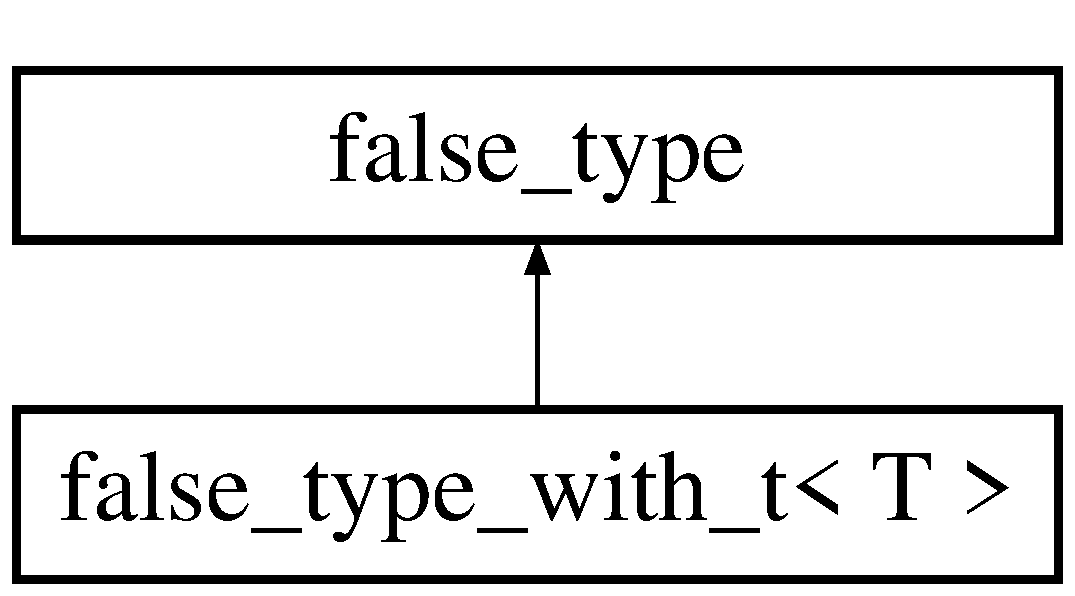
\includegraphics[height=2.000000cm]{structfalse__type__with__t}
\end{center}
\end{figure}


The documentation for this struct was generated from the following file\+:\begin{DoxyCompactItemize}
\item 
src/\hyperlink{print__ip_8hpp}{print\+\_\+ip.\+hpp}\end{DoxyCompactItemize}

\hypertarget{structis__stl__container__like}{}\section{is\+\_\+stl\+\_\+container\+\_\+like$<$ T $>$ Struct Template Reference}
\label{structis__stl__container__like}\index{is\+\_\+stl\+\_\+container\+\_\+like$<$ T $>$@{is\+\_\+stl\+\_\+container\+\_\+like$<$ T $>$}}


{\ttfamily \#include $<$is\+\_\+stl\+\_\+container\+\_\+like.\+hpp$>$}

\subsection*{Public Types}
\begin{DoxyCompactItemize}
\item 
typedef std\+::remove\+\_\+const$<$ T $>$\+::type \hyperlink{structis__stl__container__like_a4963c0bde8b0f68013b20041308b82e5}{test\+\_\+type}
\end{DoxyCompactItemize}
\subsection*{Static Public Member Functions}
\begin{DoxyCompactItemize}
\item 
{\footnotesize template$<$typename A $>$ }\\static constexpr bool \hyperlink{structis__stl__container__like_ada5dd0e7feabf4e4f7fe79db7de5d31d}{test} (A $\ast$pt, A const $\ast$cpt=nullptr, decltype(pt-\/$>$begin()) $\ast$=nullptr, decltype(pt-\/$>$end()) $\ast$=nullptr, decltype(cpt-\/$>$begin()) $\ast$=nullptr, decltype(cpt-\/$>$end()) $\ast$=nullptr, typename A\+::iterator $\ast$pi=nullptr, typename A\+::const\+\_\+iterator $\ast$pci=nullptr, typename A\+::value\+\_\+type $\ast$pv=nullptr)
\item 
{\footnotesize template$<$typename A $>$ }\\static constexpr bool \hyperlink{structis__stl__container__like_a44d72e8e872d7eb954dca89f6103e817}{test} (...)
\end{DoxyCompactItemize}
\subsection*{Static Public Attributes}
\begin{DoxyCompactItemize}
\item 
static const bool \hyperlink{structis__stl__container__like_a78703ef8497a4ebf27445e64d2eba742}{value} = \hyperlink{structis__stl__container__like_ada5dd0e7feabf4e4f7fe79db7de5d31d}{test}$<$\hyperlink{structis__stl__container__like_a4963c0bde8b0f68013b20041308b82e5}{test\+\_\+type}$>$(nullptr)
\end{DoxyCompactItemize}


\subsection{Detailed Description}
\subsubsection*{template$<$typename T$>$\newline
struct is\+\_\+stl\+\_\+container\+\_\+like$<$ T $>$}

Determine if a type is container-\/like 
\begin{DoxyTemplParams}{Template Parameters}
{\em T} & Type to be checked \\
\hline
\end{DoxyTemplParams}
\begin{DoxySeeAlso}{See also}
\href{https://stackoverflow.com/questions/9407367/determine-if-a-type-is-an-stl-container-at-compile-time}{\tt https\+://stackoverflow.\+com/questions/9407367/determine-\/if-\/a-\/type-\/is-\/an-\/stl-\/container-\/at-\/compile-\/time} 
\end{DoxySeeAlso}


\subsection{Member Typedef Documentation}
\mbox{\Hypertarget{structis__stl__container__like_a4963c0bde8b0f68013b20041308b82e5}\label{structis__stl__container__like_a4963c0bde8b0f68013b20041308b82e5}} 
\index{is\+\_\+stl\+\_\+container\+\_\+like@{is\+\_\+stl\+\_\+container\+\_\+like}!test\+\_\+type@{test\+\_\+type}}
\index{test\+\_\+type@{test\+\_\+type}!is\+\_\+stl\+\_\+container\+\_\+like@{is\+\_\+stl\+\_\+container\+\_\+like}}
\subsubsection{\texorpdfstring{test\+\_\+type}{test\_type}}
{\footnotesize\ttfamily template$<$typename T $>$ \\
typedef std\+::remove\+\_\+const$<$T$>$\+::type \hyperlink{structis__stl__container__like}{is\+\_\+stl\+\_\+container\+\_\+like}$<$ T $>$\+::\hyperlink{structis__stl__container__like_a4963c0bde8b0f68013b20041308b82e5}{test\+\_\+type}}



\subsection{Member Function Documentation}
\mbox{\Hypertarget{structis__stl__container__like_ada5dd0e7feabf4e4f7fe79db7de5d31d}\label{structis__stl__container__like_ada5dd0e7feabf4e4f7fe79db7de5d31d}} 
\index{is\+\_\+stl\+\_\+container\+\_\+like@{is\+\_\+stl\+\_\+container\+\_\+like}!test@{test}}
\index{test@{test}!is\+\_\+stl\+\_\+container\+\_\+like@{is\+\_\+stl\+\_\+container\+\_\+like}}
\subsubsection{\texorpdfstring{test()}{test()}\hspace{0.1cm}{\footnotesize\ttfamily [1/2]}}
{\footnotesize\ttfamily template$<$typename T $>$ \\
template$<$typename A $>$ \\
static constexpr bool \hyperlink{structis__stl__container__like}{is\+\_\+stl\+\_\+container\+\_\+like}$<$ T $>$\+::test (\begin{DoxyParamCaption}\item[{A $\ast$}]{pt,  }\item[{A const $\ast$}]{cpt = {\ttfamily nullptr},  }\item[{decltype(pt-\/$>$begin()) $\ast$}]{ = {\ttfamily nullptr},  }\item[{decltype(pt-\/$>$end()) $\ast$}]{ = {\ttfamily nullptr},  }\item[{decltype(cpt-\/$>$begin()) $\ast$}]{ = {\ttfamily nullptr},  }\item[{decltype(cpt-\/$>$end()) $\ast$}]{ = {\ttfamily nullptr},  }\item[{typename A\+::iterator $\ast$}]{pi = {\ttfamily nullptr},  }\item[{typename A\+::const\+\_\+iterator $\ast$}]{pci = {\ttfamily nullptr},  }\item[{typename A\+::value\+\_\+type $\ast$}]{pv = {\ttfamily nullptr} }\end{DoxyParamCaption})\hspace{0.3cm}{\ttfamily [inline]}, {\ttfamily [static]}}

\mbox{\Hypertarget{structis__stl__container__like_a44d72e8e872d7eb954dca89f6103e817}\label{structis__stl__container__like_a44d72e8e872d7eb954dca89f6103e817}} 
\index{is\+\_\+stl\+\_\+container\+\_\+like@{is\+\_\+stl\+\_\+container\+\_\+like}!test@{test}}
\index{test@{test}!is\+\_\+stl\+\_\+container\+\_\+like@{is\+\_\+stl\+\_\+container\+\_\+like}}
\subsubsection{\texorpdfstring{test()}{test()}\hspace{0.1cm}{\footnotesize\ttfamily [2/2]}}
{\footnotesize\ttfamily template$<$typename T $>$ \\
template$<$typename A $>$ \\
static constexpr bool \hyperlink{structis__stl__container__like}{is\+\_\+stl\+\_\+container\+\_\+like}$<$ T $>$\+::test (\begin{DoxyParamCaption}\item[{}]{... }\end{DoxyParamCaption})\hspace{0.3cm}{\ttfamily [inline]}, {\ttfamily [static]}}



\subsection{Member Data Documentation}
\mbox{\Hypertarget{structis__stl__container__like_a78703ef8497a4ebf27445e64d2eba742}\label{structis__stl__container__like_a78703ef8497a4ebf27445e64d2eba742}} 
\index{is\+\_\+stl\+\_\+container\+\_\+like@{is\+\_\+stl\+\_\+container\+\_\+like}!value@{value}}
\index{value@{value}!is\+\_\+stl\+\_\+container\+\_\+like@{is\+\_\+stl\+\_\+container\+\_\+like}}
\subsubsection{\texorpdfstring{value}{value}}
{\footnotesize\ttfamily template$<$typename T $>$ \\
const bool \hyperlink{structis__stl__container__like}{is\+\_\+stl\+\_\+container\+\_\+like}$<$ T $>$\+::value = \hyperlink{structis__stl__container__like_ada5dd0e7feabf4e4f7fe79db7de5d31d}{test}$<$\hyperlink{structis__stl__container__like_a4963c0bde8b0f68013b20041308b82e5}{test\+\_\+type}$>$(nullptr)\hspace{0.3cm}{\ttfamily [static]}}



The documentation for this struct was generated from the following file\+:\begin{DoxyCompactItemize}
\item 
src/\hyperlink{is__stl__container__like_8hpp}{is\+\_\+stl\+\_\+container\+\_\+like.\+hpp}\end{DoxyCompactItemize}

\hypertarget{structis__string}{}\section{is\+\_\+string$<$ T, typename $>$ Struct Template Reference}
\label{structis__string}\index{is\+\_\+string$<$ T, typename $>$@{is\+\_\+string$<$ T, typename $>$}}


{\ttfamily \#include $<$is\+\_\+string.\+hpp$>$}

\subsection*{Static Public Attributes}
\begin{DoxyCompactItemize}
\item 
static constexpr bool \hyperlink{structis__string_a3832f7471ae89c5903a6242e4e2517d7}{value} = false
\end{DoxyCompactItemize}


\subsection{Member Data Documentation}
\mbox{\Hypertarget{structis__string_a3832f7471ae89c5903a6242e4e2517d7}\label{structis__string_a3832f7471ae89c5903a6242e4e2517d7}} 
\index{is\+\_\+string@{is\+\_\+string}!value@{value}}
\index{value@{value}!is\+\_\+string@{is\+\_\+string}}
\subsubsection{\texorpdfstring{value}{value}}
{\footnotesize\ttfamily template$<$typename T , typename  = void$>$ \\
constexpr bool \hyperlink{structis__string}{is\+\_\+string}$<$ T, typename $>$\+::value = false\hspace{0.3cm}{\ttfamily [static]}}



The documentation for this struct was generated from the following file\+:\begin{DoxyCompactItemize}
\item 
src/\hyperlink{is__string_8hpp}{is\+\_\+string.\+hpp}\end{DoxyCompactItemize}

\hypertarget{structis__string_3_01std_1_1basic__string_3_01T_00_01Traits_00_01Alloc_01_4_00_01void_01_4}{}\section{is\+\_\+string$<$ std\+:\+:basic\+\_\+string$<$ T, Traits, Alloc $>$, void $>$ Struct Template Reference}
\label{structis__string_3_01std_1_1basic__string_3_01T_00_01Traits_00_01Alloc_01_4_00_01void_01_4}\index{is\+\_\+string$<$ std\+::basic\+\_\+string$<$ T, Traits, Alloc $>$, void $>$@{is\+\_\+string$<$ std\+::basic\+\_\+string$<$ T, Traits, Alloc $>$, void $>$}}


{\ttfamily \#include $<$is\+\_\+string.\+hpp$>$}

\subsection*{Static Public Attributes}
\begin{DoxyCompactItemize}
\item 
static constexpr bool \hyperlink{structis__string_3_01std_1_1basic__string_3_01T_00_01Traits_00_01Alloc_01_4_00_01void_01_4_ad067ab285d00dda3bf3ef0d9dd3bedac}{value} = true
\end{DoxyCompactItemize}


\subsection{Member Data Documentation}
\mbox{\Hypertarget{structis__string_3_01std_1_1basic__string_3_01T_00_01Traits_00_01Alloc_01_4_00_01void_01_4_ad067ab285d00dda3bf3ef0d9dd3bedac}\label{structis__string_3_01std_1_1basic__string_3_01T_00_01Traits_00_01Alloc_01_4_00_01void_01_4_ad067ab285d00dda3bf3ef0d9dd3bedac}} 
\index{is\+\_\+string$<$ std\+::basic\+\_\+string$<$ T, Traits, Alloc $>$, void $>$@{is\+\_\+string$<$ std\+::basic\+\_\+string$<$ T, Traits, Alloc $>$, void $>$}!value@{value}}
\index{value@{value}!is\+\_\+string$<$ std\+::basic\+\_\+string$<$ T, Traits, Alloc $>$, void $>$@{is\+\_\+string$<$ std\+::basic\+\_\+string$<$ T, Traits, Alloc $>$, void $>$}}
\subsubsection{\texorpdfstring{value}{value}}
{\footnotesize\ttfamily template$<$typename T , class Traits , class Alloc $>$ \\
constexpr bool \hyperlink{structis__string}{is\+\_\+string}$<$ std\+::basic\+\_\+string$<$ T, Traits, Alloc $>$, void $>$\+::value = true\hspace{0.3cm}{\ttfamily [static]}}



The documentation for this struct was generated from the following file\+:\begin{DoxyCompactItemize}
\item 
src/\hyperlink{is__string_8hpp}{is\+\_\+string.\+hpp}\end{DoxyCompactItemize}

\hypertarget{structis__uniform__tuple}{}\section{is\+\_\+uniform\+\_\+tuple$<$ T, typename $>$ Struct Template Reference}
\label{structis__uniform__tuple}\index{is\+\_\+uniform\+\_\+tuple$<$ T, typename $>$@{is\+\_\+uniform\+\_\+tuple$<$ T, typename $>$}}


{\ttfamily \#include $<$is\+\_\+uniform\+\_\+tuple.\+hpp$>$}

\subsection*{Static Public Attributes}
\begin{DoxyCompactItemize}
\item 
static constexpr bool \hyperlink{structis__uniform__tuple_a3ba254c18d5af79286118c59003d529e}{value} = false
\end{DoxyCompactItemize}


\subsection{Member Data Documentation}
\mbox{\Hypertarget{structis__uniform__tuple_a3ba254c18d5af79286118c59003d529e}\label{structis__uniform__tuple_a3ba254c18d5af79286118c59003d529e}} 
\index{is\+\_\+uniform\+\_\+tuple@{is\+\_\+uniform\+\_\+tuple}!value@{value}}
\index{value@{value}!is\+\_\+uniform\+\_\+tuple@{is\+\_\+uniform\+\_\+tuple}}
\subsubsection{\texorpdfstring{value}{value}}
{\footnotesize\ttfamily template$<$typename T, typename  = void$>$ \\
constexpr bool \hyperlink{structis__uniform__tuple}{is\+\_\+uniform\+\_\+tuple}$<$ T, typename $>$\+::value = false\hspace{0.3cm}{\ttfamily [static]}}



The documentation for this struct was generated from the following file\+:\begin{DoxyCompactItemize}
\item 
src/\hyperlink{is__uniform__tuple_8hpp}{is\+\_\+uniform\+\_\+tuple.\+hpp}\end{DoxyCompactItemize}

\hypertarget{structis__uniform__tuple_3_01std_1_1tuple_3_01Ts_8_8_8_01_4_01_4}{}\section{is\+\_\+uniform\+\_\+tuple$<$ std\+:\+:tuple$<$ Ts... $>$ $>$ Struct Template Reference}
\label{structis__uniform__tuple_3_01std_1_1tuple_3_01Ts_8_8_8_01_4_01_4}\index{is\+\_\+uniform\+\_\+tuple$<$ std\+::tuple$<$ Ts... $>$ $>$@{is\+\_\+uniform\+\_\+tuple$<$ std\+::tuple$<$ Ts... $>$ $>$}}


{\ttfamily \#include $<$is\+\_\+uniform\+\_\+tuple.\+hpp$>$}

\subsection*{Static Public Attributes}
\begin{DoxyCompactItemize}
\item 
static constexpr bool \hyperlink{structis__uniform__tuple_3_01std_1_1tuple_3_01Ts_8_8_8_01_4_01_4_ae218f20e67acacb3596b3247ffd7438c}{value} = \hyperlink{is__uniform__tuple_8hpp_a8f9339dd3f878ad76e81f7a03785284d}{is\+\_\+same\+\_\+all\+\_\+v}$<$Ts...$>$
\end{DoxyCompactItemize}


\subsection{Member Data Documentation}
\mbox{\Hypertarget{structis__uniform__tuple_3_01std_1_1tuple_3_01Ts_8_8_8_01_4_01_4_ae218f20e67acacb3596b3247ffd7438c}\label{structis__uniform__tuple_3_01std_1_1tuple_3_01Ts_8_8_8_01_4_01_4_ae218f20e67acacb3596b3247ffd7438c}} 
\index{is\+\_\+uniform\+\_\+tuple$<$ std\+::tuple$<$ Ts... $>$ $>$@{is\+\_\+uniform\+\_\+tuple$<$ std\+::tuple$<$ Ts... $>$ $>$}!value@{value}}
\index{value@{value}!is\+\_\+uniform\+\_\+tuple$<$ std\+::tuple$<$ Ts... $>$ $>$@{is\+\_\+uniform\+\_\+tuple$<$ std\+::tuple$<$ Ts... $>$ $>$}}
\subsubsection{\texorpdfstring{value}{value}}
{\footnotesize\ttfamily template$<$typename... Ts$>$ \\
constexpr bool \hyperlink{structis__uniform__tuple}{is\+\_\+uniform\+\_\+tuple}$<$ std\+::tuple$<$ Ts... $>$ $>$\+::value = \hyperlink{is__uniform__tuple_8hpp_a8f9339dd3f878ad76e81f7a03785284d}{is\+\_\+same\+\_\+all\+\_\+v}$<$Ts...$>$\hspace{0.3cm}{\ttfamily [static]}}



The documentation for this struct was generated from the following file\+:\begin{DoxyCompactItemize}
\item 
src/\hyperlink{is__uniform__tuple_8hpp}{is\+\_\+uniform\+\_\+tuple.\+hpp}\end{DoxyCompactItemize}

\chapter{File Documentation}
\hypertarget{CMakeLists_8txt}{}\section{src/\+C\+Make\+Lists.txt File Reference}
\label{CMakeLists_8txt}\index{src/\+C\+Make\+Lists.\+txt@{src/\+C\+Make\+Lists.\+txt}}

\hypertarget{is__stl__container__like_8hpp}{}\section{src/is\+\_\+stl\+\_\+container\+\_\+like.hpp File Reference}
\label{is__stl__container__like_8hpp}\index{src/is\+\_\+stl\+\_\+container\+\_\+like.\+hpp@{src/is\+\_\+stl\+\_\+container\+\_\+like.\+hpp}}
{\ttfamily \#include $<$type\+\_\+traits$>$}\newline
\subsection*{Classes}
\begin{DoxyCompactItemize}
\item 
struct \hyperlink{structis__stl__container__like}{is\+\_\+stl\+\_\+container\+\_\+like$<$ T $>$}
\end{DoxyCompactItemize}
\subsection*{Variables}
\begin{DoxyCompactItemize}
\item 
{\footnotesize template$<$typename T $>$ }\\constexpr bool \hyperlink{is__stl__container__like_8hpp_ae00a2896a146a68d911c7e7b4ccaab78}{is\+\_\+stl\+\_\+container\+\_\+like\+\_\+v} = \hyperlink{structis__stl__container__like}{is\+\_\+stl\+\_\+container\+\_\+like}$<$T$>$\+::value
\end{DoxyCompactItemize}


\subsection{Variable Documentation}
\mbox{\Hypertarget{is__stl__container__like_8hpp_ae00a2896a146a68d911c7e7b4ccaab78}\label{is__stl__container__like_8hpp_ae00a2896a146a68d911c7e7b4ccaab78}} 
\index{is\+\_\+stl\+\_\+container\+\_\+like.\+hpp@{is\+\_\+stl\+\_\+container\+\_\+like.\+hpp}!is\+\_\+stl\+\_\+container\+\_\+like\+\_\+v@{is\+\_\+stl\+\_\+container\+\_\+like\+\_\+v}}
\index{is\+\_\+stl\+\_\+container\+\_\+like\+\_\+v@{is\+\_\+stl\+\_\+container\+\_\+like\+\_\+v}!is\+\_\+stl\+\_\+container\+\_\+like.\+hpp@{is\+\_\+stl\+\_\+container\+\_\+like.\+hpp}}
\subsubsection{\texorpdfstring{is\+\_\+stl\+\_\+container\+\_\+like\+\_\+v}{is\_stl\_container\_like\_v}}
{\footnotesize\ttfamily template$<$typename T $>$ \\
constexpr bool is\+\_\+stl\+\_\+container\+\_\+like\+\_\+v = \hyperlink{structis__stl__container__like}{is\+\_\+stl\+\_\+container\+\_\+like}$<$T$>$\+::value}


\hypertarget{is__string_8hpp}{}\section{src/is\+\_\+string.hpp File Reference}
\label{is__string_8hpp}\index{src/is\+\_\+string.\+hpp@{src/is\+\_\+string.\+hpp}}


Helper types.  


{\ttfamily \#include $<$string$>$}\newline
\subsection*{Classes}
\begin{DoxyCompactItemize}
\item 
struct \hyperlink{structis__string}{is\+\_\+string$<$ T, typename $>$}
\item 
struct \hyperlink{structis__string_3_01std_1_1basic__string_3_01T_00_01Traits_00_01Alloc_01_4_00_01void_01_4}{is\+\_\+string$<$ std\+::basic\+\_\+string$<$ T, Traits, Alloc $>$, void $>$}
\end{DoxyCompactItemize}
\subsection*{Variables}
\begin{DoxyCompactItemize}
\item 
{\footnotesize template$<$typename T $>$ }\\constexpr bool \hyperlink{is__string_8hpp_a86a2e3fab8ec3012c24e41f2ad073cf9}{is\+\_\+string\+\_\+v} = \hyperlink{structis__string}{is\+\_\+string}$<$T$>$\+::value
\item 
{\footnotesize template$<$typename T $>$ }\\constexpr bool \hyperlink{is__string_8hpp_a7e68b78bf5e32fedaa954e5315d0e73c}{is\+\_\+c\+\_\+string\+\_\+v}
\end{DoxyCompactItemize}


\subsection{Detailed Description}
Helper types. 



\subsection{Variable Documentation}
\mbox{\Hypertarget{is__string_8hpp_a7e68b78bf5e32fedaa954e5315d0e73c}\label{is__string_8hpp_a7e68b78bf5e32fedaa954e5315d0e73c}} 
\index{is\+\_\+string.\+hpp@{is\+\_\+string.\+hpp}!is\+\_\+c\+\_\+string\+\_\+v@{is\+\_\+c\+\_\+string\+\_\+v}}
\index{is\+\_\+c\+\_\+string\+\_\+v@{is\+\_\+c\+\_\+string\+\_\+v}!is\+\_\+string.\+hpp@{is\+\_\+string.\+hpp}}
\subsubsection{\texorpdfstring{is\+\_\+c\+\_\+string\+\_\+v}{is\_c\_string\_v}}
{\footnotesize\ttfamily template$<$typename T $>$ \\
constexpr bool is\+\_\+c\+\_\+string\+\_\+v}

{\bfseries Initial value\+:}
\begin{DoxyCode}
= std::is\_same\_v<\textcolor{keywordtype}{char}*,
                                              std::remove\_reference\_t<
                                                  std::remove\_cv\_t<
                                                      std::decay\_t<T>
                                                  >
                                              >
>
\end{DoxyCode}
\mbox{\Hypertarget{is__string_8hpp_a86a2e3fab8ec3012c24e41f2ad073cf9}\label{is__string_8hpp_a86a2e3fab8ec3012c24e41f2ad073cf9}} 
\index{is\+\_\+string.\+hpp@{is\+\_\+string.\+hpp}!is\+\_\+string\+\_\+v@{is\+\_\+string\+\_\+v}}
\index{is\+\_\+string\+\_\+v@{is\+\_\+string\+\_\+v}!is\+\_\+string.\+hpp@{is\+\_\+string.\+hpp}}
\subsubsection{\texorpdfstring{is\+\_\+string\+\_\+v}{is\_string\_v}}
{\footnotesize\ttfamily template$<$typename T $>$ \\
constexpr bool is\+\_\+string\+\_\+v = \hyperlink{structis__string}{is\+\_\+string}$<$T$>$\+::value}


\hypertarget{is__uniform__tuple_8hpp}{}\section{src/is\+\_\+uniform\+\_\+tuple.hpp File Reference}
\label{is__uniform__tuple_8hpp}\index{src/is\+\_\+uniform\+\_\+tuple.\+hpp@{src/is\+\_\+uniform\+\_\+tuple.\+hpp}}
{\ttfamily \#include $<$tuple$>$}\newline
{\ttfamily \#include $<$type\+\_\+traits$>$}\newline
\subsection*{Classes}
\begin{DoxyCompactItemize}
\item 
struct \hyperlink{structis__uniform__tuple}{is\+\_\+uniform\+\_\+tuple$<$ T, typename $>$}
\item 
struct \hyperlink{structis__uniform__tuple_3_01std_1_1tuple_3_01Ts_8_8_8_01_4_01_4}{is\+\_\+uniform\+\_\+tuple$<$ std\+::tuple$<$ Ts... $>$ $>$}
\end{DoxyCompactItemize}
\subsection*{Variables}
\begin{DoxyCompactItemize}
\item 
{\footnotesize template$<$typename T , typename... Ts$>$ }\\constexpr bool \hyperlink{is__uniform__tuple_8hpp_a8f9339dd3f878ad76e81f7a03785284d}{is\+\_\+same\+\_\+all\+\_\+v} = std\+::conjunction\+\_\+v$<$std\+::is\+\_\+same$<$T, Ts$>$...$>$
\item 
{\footnotesize template$<$typename T $>$ }\\constexpr bool \hyperlink{is__uniform__tuple_8hpp_a7bce08af2c229ebd49e1419ef9bb518b}{is\+\_\+uniform\+\_\+tuple\+\_\+v} = \hyperlink{structis__uniform__tuple}{is\+\_\+uniform\+\_\+tuple}$<$std\+::remove\+\_\+const\+\_\+t$<$std\+::remove\+\_\+cv\+\_\+t$<$T$>$$>$$>$\+::value
\end{DoxyCompactItemize}


\subsection{Variable Documentation}
\mbox{\Hypertarget{is__uniform__tuple_8hpp_a8f9339dd3f878ad76e81f7a03785284d}\label{is__uniform__tuple_8hpp_a8f9339dd3f878ad76e81f7a03785284d}} 
\index{is\+\_\+uniform\+\_\+tuple.\+hpp@{is\+\_\+uniform\+\_\+tuple.\+hpp}!is\+\_\+same\+\_\+all\+\_\+v@{is\+\_\+same\+\_\+all\+\_\+v}}
\index{is\+\_\+same\+\_\+all\+\_\+v@{is\+\_\+same\+\_\+all\+\_\+v}!is\+\_\+uniform\+\_\+tuple.\+hpp@{is\+\_\+uniform\+\_\+tuple.\+hpp}}
\subsubsection{\texorpdfstring{is\+\_\+same\+\_\+all\+\_\+v}{is\_same\_all\_v}}
{\footnotesize\ttfamily template$<$typename T , typename... Ts$>$ \\
constexpr bool is\+\_\+same\+\_\+all\+\_\+v = std\+::conjunction\+\_\+v$<$std\+::is\+\_\+same$<$T, Ts$>$...$>$}

\mbox{\Hypertarget{is__uniform__tuple_8hpp_a7bce08af2c229ebd49e1419ef9bb518b}\label{is__uniform__tuple_8hpp_a7bce08af2c229ebd49e1419ef9bb518b}} 
\index{is\+\_\+uniform\+\_\+tuple.\+hpp@{is\+\_\+uniform\+\_\+tuple.\+hpp}!is\+\_\+uniform\+\_\+tuple\+\_\+v@{is\+\_\+uniform\+\_\+tuple\+\_\+v}}
\index{is\+\_\+uniform\+\_\+tuple\+\_\+v@{is\+\_\+uniform\+\_\+tuple\+\_\+v}!is\+\_\+uniform\+\_\+tuple.\+hpp@{is\+\_\+uniform\+\_\+tuple.\+hpp}}
\subsubsection{\texorpdfstring{is\+\_\+uniform\+\_\+tuple\+\_\+v}{is\_uniform\_tuple\_v}}
{\footnotesize\ttfamily template$<$typename T $>$ \\
constexpr bool is\+\_\+uniform\+\_\+tuple\+\_\+v = \hyperlink{structis__uniform__tuple}{is\+\_\+uniform\+\_\+tuple}$<$std\+::remove\+\_\+const\+\_\+t$<$std\+::remove\+\_\+cv\+\_\+t$<$T$>$$>$$>$\+::value}

Checks if type is a tuple with uniform parameter types 
\begin{DoxyTemplParams}{Template Parameters}
{\em T} & Type to be checked \\
\hline
\end{DoxyTemplParams}

\hypertarget{main_8cpp}{}\section{src/main.cpp File Reference}
\label{main_8cpp}\index{src/main.\+cpp@{src/main.\+cpp}}
\subsection*{Functions}
\begin{DoxyCompactItemize}
\item 
int \hyperlink{main_8cpp_ae66f6b31b5ad750f1fe042a706a4e3d4}{main} ()
\end{DoxyCompactItemize}


\subsection{Function Documentation}
\mbox{\Hypertarget{main_8cpp_ae66f6b31b5ad750f1fe042a706a4e3d4}\label{main_8cpp_ae66f6b31b5ad750f1fe042a706a4e3d4}} 
\index{main.\+cpp@{main.\+cpp}!main@{main}}
\index{main@{main}!main.\+cpp@{main.\+cpp}}
\subsubsection{\texorpdfstring{main()}{main()}}
{\footnotesize\ttfamily int main (\begin{DoxyParamCaption}{ }\end{DoxyParamCaption})}


\hypertarget{print__ip_8hpp}{}\section{src/print\+\_\+ip.hpp File Reference}
\label{print__ip_8hpp}\index{src/print\+\_\+ip.\+hpp@{src/print\+\_\+ip.\+hpp}}


Contains print\+\_\+ip function.  


{\ttfamily \#include \char`\"{}is\+\_\+stl\+\_\+container\+\_\+like.\+hpp\char`\"{}}\newline
{\ttfamily \#include \char`\"{}is\+\_\+string.\+hpp\char`\"{}}\newline
{\ttfamily \#include \char`\"{}is\+\_\+uniform\+\_\+tuple.\+hpp\char`\"{}}\newline
{\ttfamily \#include \char`\"{}static\+\_\+for.\+hpp\char`\"{}}\newline
{\ttfamily \#include $<$type\+\_\+traits$>$}\newline
{\ttfamily \#include $<$iostream$>$}\newline
{\ttfamily \#include $<$utility$>$}\newline
\subsection*{Classes}
\begin{DoxyCompactItemize}
\item 
struct \hyperlink{structfalse__type__with__t}{false\+\_\+type\+\_\+with\+\_\+t$<$ T $>$}
\end{DoxyCompactItemize}
\subsection*{Functions}
\begin{DoxyCompactItemize}
\item 
{\footnotesize template$<$typename T $>$ }\\void \hyperlink{print__ip_8hpp_ac0f0648810109c3328aac0386d23faba}{print\+\_\+ip} (const T \&data, std\+::ostream \&stream=std\+::cout)
\end{DoxyCompactItemize}


\subsection{Detailed Description}
Contains print\+\_\+ip function. 



\subsection{Function Documentation}
\mbox{\Hypertarget{print__ip_8hpp_ac0f0648810109c3328aac0386d23faba}\label{print__ip_8hpp_ac0f0648810109c3328aac0386d23faba}} 
\index{print\+\_\+ip.\+hpp@{print\+\_\+ip.\+hpp}!print\+\_\+ip@{print\+\_\+ip}}
\index{print\+\_\+ip@{print\+\_\+ip}!print\+\_\+ip.\+hpp@{print\+\_\+ip.\+hpp}}
\subsubsection{\texorpdfstring{print\+\_\+ip()}{print\_ip()}}
{\footnotesize\ttfamily template$<$typename T $>$ \\
void print\+\_\+ip (\begin{DoxyParamCaption}\item[{const T \&}]{data,  }\item[{std\+::ostream \&}]{stream = {\ttfamily std\+:\+:cout} }\end{DoxyParamCaption})}

Print an IP to stream 
\begin{DoxyTemplParams}{Template Parameters}
{\em T} & \\
\hline
\end{DoxyTemplParams}

\begin{DoxyParams}{Parameters}
{\em stream} & Stream to write to \\
\hline
{\em data} & IP address \\
\hline
\end{DoxyParams}

\hypertarget{static__for_8hpp}{}\section{src/static\+\_\+for.hpp File Reference}
\label{static__for_8hpp}\index{src/static\+\_\+for.\+hpp@{src/static\+\_\+for.\+hpp}}
{\ttfamily \#include $<$utility$>$}\newline
\subsection*{Functions}
\begin{DoxyCompactItemize}
\item 
{\footnotesize template$<$class Tup , class Func , std\+::size\+\_\+t ... Is$>$ }\\constexpr void \hyperlink{static__for_8hpp_aa52c2cc34b6400b3c7a5e2f323b6eef9}{static\+\_\+for\+\_\+impl} (Tup \&\&t, Func \&\&f, std\+::index\+\_\+sequence$<$ Is... $>$)
\item 
{\footnotesize template$<$class ... T, class Func $>$ }\\constexpr void \hyperlink{static__for_8hpp_ae37d6ad4f6fd3442600b3c01fc093eef}{static\+\_\+for} (const std\+::tuple$<$ T... $>$ \&t, Func \&\&f)
\end{DoxyCompactItemize}


\subsection{Function Documentation}
\mbox{\Hypertarget{static__for_8hpp_ae37d6ad4f6fd3442600b3c01fc093eef}\label{static__for_8hpp_ae37d6ad4f6fd3442600b3c01fc093eef}} 
\index{static\+\_\+for.\+hpp@{static\+\_\+for.\+hpp}!static\+\_\+for@{static\+\_\+for}}
\index{static\+\_\+for@{static\+\_\+for}!static\+\_\+for.\+hpp@{static\+\_\+for.\+hpp}}
\subsubsection{\texorpdfstring{static\+\_\+for()}{static\_for()}}
{\footnotesize\ttfamily template$<$class ... T, class Func $>$ \\
constexpr void static\+\_\+for (\begin{DoxyParamCaption}\item[{const std\+::tuple$<$ T... $>$ \&}]{t,  }\item[{Func \&\&}]{f }\end{DoxyParamCaption})}

Helper function to iterate over a tuple 
\begin{DoxyTemplParams}{Template Parameters}
{\em T} & Tuple type arguments \\
\hline
{\em Func} & Function type \\
\hline
\end{DoxyTemplParams}

\begin{DoxyParams}{Parameters}
{\em t} & Tuple \\
\hline
{\em f} & Function \\
\hline
\end{DoxyParams}
\mbox{\Hypertarget{static__for_8hpp_aa52c2cc34b6400b3c7a5e2f323b6eef9}\label{static__for_8hpp_aa52c2cc34b6400b3c7a5e2f323b6eef9}} 
\index{static\+\_\+for.\+hpp@{static\+\_\+for.\+hpp}!static\+\_\+for\+\_\+impl@{static\+\_\+for\+\_\+impl}}
\index{static\+\_\+for\+\_\+impl@{static\+\_\+for\+\_\+impl}!static\+\_\+for.\+hpp@{static\+\_\+for.\+hpp}}
\subsubsection{\texorpdfstring{static\+\_\+for\+\_\+impl()}{static\_for\_impl()}}
{\footnotesize\ttfamily template$<$class Tup , class Func , std\+::size\+\_\+t ... Is$>$ \\
constexpr void static\+\_\+for\+\_\+impl (\begin{DoxyParamCaption}\item[{Tup \&\&}]{t,  }\item[{Func \&\&}]{f,  }\item[{std\+::index\+\_\+sequence$<$ Is... $>$}]{ }\end{DoxyParamCaption})}


%--- End generated contents ---

% Index
\backmatter
\newpage
\phantomsection
\clearemptydoublepage
\addcontentsline{toc}{chapter}{Index}
\printindex

\end{document}
